%% swarm-abm — manuscript for Simulation Modelling Practice and Theory (SIMPAT)
%% Elsevier elsarticle class. Submission format: [review] (single column,
%% double spaced, line numbers). Final two-column look: replace with [5p].
\documentclass[review]{elsarticle}

\usepackage{lineno}
\usepackage{amsmath}
\usepackage{booktabs}
\usepackage{graphicx}
\usepackage[hidelinks]{hyperref}
\modulolinenumbers[5]

\journal{Simulation Modelling Practice and Theory}
\bibliographystyle{elsarticle-num}

\begin{document}

\begin{frontmatter}

\title{Determinism by construction: reproducible parallelism in swarm-abm,
a multi-paradigm engine for spatial agent-based simulation}

%% TODO: author names, affiliations, corresponding author
\author[a]{First Author\corref{cor1}}
\ead{author@example.org}
\cortext[cor1]{Corresponding author}
\affiliation[a]{organization={Affiliation},
            city={City},
            country={Country}}

\begin{abstract}
Reproducibility is foundational to computational science. Yet agent-based
modelling (ABM), a workhorse across ecology, epidemiology, the social sciences
and the geosciences, is typically practised on platforms (NetLogo, Mesa) that
rely on global, unseeded randomness. Such platforms cannot guarantee that a
result reproduces bit-for-bit, across machines, or as parallelism is added. We
present swarm-abm, a spatial ABM engine in Rust built around \emph{determinism
by construction}. A single agent/model API spans three spatial paradigms (grid,
network, continuous space) over a seedable, portable generator. The engine's
central mechanism is a two-phase synchronous update whose decision phase
receives the model immutably. The type system therefore proves that no agent
mutates shared state during decision. This removes the read-after-write hazard
of synchronous ABM by construction, a verification guarantee rather than a
convention, and makes the decision phase safe to parallelise. Paired with a
per-agent generator keyed on $(\text{seed},\text{step},\text{agent})$, parallel
execution is bit-for-bit identical to sequential, independent of thread count.
We validate the generator with PractRand and confirm identical results across
x86-64 and WebAssembly. On spatial SIR and Schelling, swarm-abm runs
2--5$\times$ faster single-threaded than Agents.jl, the fastest compiled ABM
framework, and 45--184$\times$ faster than Mesa. The parallel decision phase
scales about fivefold on 16 cores for compute-bound decisions. A debris-flow
application shows this throughput turning an infeasible study, a powered
comparison of five metaheuristic calibrators, into a routine one. Python
bindings and a WebAssembly viewer are provided; the engine is open source.
\end{abstract}

\begin{keyword}
agent-based modelling \sep simulation framework \sep reproducibility \sep
parallel simulation \sep verification and validation \sep Rust
\end{keyword}

\end{frontmatter}

\linenumbers

\section{Introduction}
\label{sec:intro}

Agent-based modelling (ABM) builds system-level behaviour from the bottom up,
out of local interactions among many heterogeneous agents, and is a standard
method across ecology, epidemiology, the social sciences and the geosciences.
Because an ABM is a stochastic computational experiment, its scientific value
rests on \emph{reproducibility}: the same model, inputs and seed should yield
the same result, on any machine, and whether it runs on one thread or many.
Yet the two platforms that dominate practice fall short of this bar. NetLogo
\cite{wilensky1999netlogo}, on the Java virtual machine, and Mesa
\cite{kazil2020mesa}, in Python, both lean on a global, unseeded random source
by default, so results are difficult to reproduce bit-for-bit; neither offers a
cross-platform or parallel reproducibility guarantee.

Reproducibility is not the only casualty. \emph{The cost of a single run shapes
the science that gets done.} When one replicate of a spatial model takes
minutes, studies default to a single run per condition, calibrations are tuned
to a single random seed (and silently overfit it), and sensitivity analyses are
truncated. These methodological compromises are invisible in the published
result. A faster engine does not merely save wall-clock time; it widens the
space of experimental designs that are feasible at all.

We identify three gaps in current spatial ABM tooling, and a fourth concern
specific to \emph{synchronous} (simultaneous) update. (1)
\textbf{Reproducibility}: reliance on global, unseeded randomness undermines
bit-level replication. (2) \textbf{Performance}: the per-run cost forces the
impoverished experimental designs noted above. (3) \textbf{Spatial generality}:
tools tend to privilege one spatial paradigm, so moving a question from a grid
to a network to a continuous space typically means a rewrite. (4) The
\textbf{synchronous-update hazard}: in two-phase (decide/apply) update, every
agent must decide against the \emph{same} snapshot of the world; if any agent
reads a neighbour's freshly written state during the decision phase
(read-after-write), the update is silently corrupted. In existing frameworks
this is a matter of user discipline, not a guarantee.

This paper presents \textbf{swarm-abm}, a spatial ABM engine written in Rust
whose organising principle is \emph{determinism by construction}, and whose
sharp technical kernel is a type-enforced immutability that serves two ends at
once: it \emph{proves} the synchronous update correct, and it is exactly what
makes that update safe to parallelise without sacrificing bit-level
reproducibility. Concretely, our contributions are:

\begin{itemize}
  \item A \textbf{multi-paradigm engine} exposing a regular grid, a network
  (graph) and a continuous space under one \texttt{Agent}/\texttt{Model} API,
  over a seedable, portable, bit-for-bit deterministic generator
  (Section~\ref{sec:design}).
  \item A \textbf{compiler-verified synchronous update}: the decision phase
  receives the model immutably, so the type system proves that no agent writes
  shared state during decision. This removes read-after-write by construction
  (a verification guarantee, not a convention) and is precisely what makes the
  phase safe to parallelise (Section~\ref{sec:sync}).
  \item \textbf{Deterministic parallelism}: a per-agent generator keyed on
  $(\text{seed},\text{step},\text{agent})$ renders parallel execution
  bit-for-bit identical to sequential, independent of thread count. We validate
  the generator with PractRand and confirm bit-identical results across x86-64
  and WebAssembly (Section~\ref{sec:vv}).
  \item A \textbf{performance evaluation against the real peers}: on spatial SIR
  and Schelling, swarm-abm is 2--5$\times$ faster single-threaded than
  Agents.jl \cite{datseris2022agents}, the fastest compiled ABM framework,
  and 45--184$\times$ faster than Mesa; the parallel decision phase scales
  $\sim$5$\times$ on 16 cores when per-agent decisions are compute-bound
  (Section~\ref{sec:perf}).
  \item A \textbf{real-world demonstration} in which the engine's throughput
  turns a previously infeasible study (a statistically powered comparison of
  five metaheuristic calibrators) into a routine one
  (Section~\ref{sec:app}), plus Python bindings and a WebAssembly viewer
  (Section~\ref{sec:access}).
\end{itemize}

The remainder of the paper is organised as follows.
Section~\ref{sec:design} describes the engine. Section~\ref{sec:sync} develops
the synchronous-update guarantee and deterministic parallelism.
Section~\ref{sec:vv} reports verification and validation.
Section~\ref{sec:perf} reports performance and scalability.
Section~\ref{sec:app} presents the application. Section~\ref{sec:access} covers
accessibility and reproducibility. Sections~\ref{sec:discussion}
and~\ref{sec:conclusion} discuss and conclude.

\section{Engine design}
\label{sec:design}

\subsection{Agents and models}
A swarm-abm model owns its agents and any spatial environment. Agents implement
an \texttt{Agent} trait and the global state implements a \texttt{Model} trait;
the engine drives them through a fixed per-step protocol (environment update,
agent activation in scheduler order, post-step bookkeeping, data collection).
The central design problem is that an agent's behaviour needs mutable access to
itself \emph{and} read/write access to the rest of the model (including other
agents) at the same time, a borrow conflict in a language with compile-time
aliasing rules. swarm-abm resolves this with a \emph{take-out} pattern: while an
agent runs, it is temporarily removed from the model's agent set, so it can be
handed full mutable access to the model with no aliasing, and is returned
afterwards. This avoids interior-mutability escape hatches and keeps the hot
path allocation-free (the activation-order buffer is reused across steps).

\subsection{Three spatial paradigms, one API}
The same \texttt{Agent}/\texttt{Model} abstraction hosts three spatial
structures. \texttt{Grid2D} is a dense 2-D lattice with Moore and Von Neumann
neighbourhoods, optional toroidal wrapping, and a NetLogo-style \texttt{diffuse}
operator. \texttt{Graph} is a topological space with deterministic generators
for Erd\H{o}s--R\'enyi, Watts--Strogatz (small-world) and Barab\'asi--Albert
(scale-free) networks. \texttt{ContinuousSpace} is an off-lattice space with
radius queries accelerated by spatial hashing and no per-query allocation.
Moving a model between paradigms reuses the same agent logic and scheduler;
only the spatial queries change.

\subsection{Scheduling}
Activation policy is explicit: \texttt{Ordered} (insertion order),
\texttt{Random} (a fresh seeded permutation each step, the ABM default for
avoiding order artefacts), or \texttt{Simultaneous} (the two-phase synchronous
update of Section~\ref{sec:sync}). A model written in the two-phase style also
runs under sequential policies, so the same code can be exercised both ways.

\subsection{Determinism and data collection}
All randomness flows through \texttt{SimRng}, a seedable ChaCha8 generator
\cite{bernstein2008chacha} that produces the same stream for a given seed on
any platform and across versions of the underlying numeric libraries; models
never touch a global generator. A \texttt{DataCollector} records per-step
scalar series for later export. Determinism is thus a property of the engine,
not of user discipline.

\subsection{Batch execution}
Replicates and parameter sweeps, the bread and butter of an ABM study, are
first-class: \texttt{run\_ensemble} and \texttt{run\_sweep} evaluate a model
over many seeds and configurations and reduce each run to a summary. With the
\texttt{parallel} feature these distribute across cores via a work-stealing
pool; without it (e.g.\ for WebAssembly) they run sequentially. Because each run
is fully seeded, ensemble results are themselves reproducible.

\section{Synchronous update as a verification guarantee, and deterministic parallelism}
\label{sec:sync}

\subsection{The read-after-write hazard}
In synchronous (simultaneous) update, time advances in two phases. In the
\emph{decision} phase every agent computes its next state from the
\emph{current} world; in the \emph{apply} phase every agent commits that next
state. The defining requirement is that all agents decide against one
consistent snapshot. If, during decision, an agent reads a neighbour that has
already written its \emph{next} state, the snapshot is no longer consistent and
the update is silently wrong, a classic and easily introduced verification
defect. In NetLogo, Mesa, Repast and Agents.jl this correctness condition is
maintained by user discipline (writing to a separate ``next'' field, or reading
from a hand-built snapshot); nothing in the tooling prevents a violation.

\subsection{A guarantee from the type system}
swarm-abm makes the condition a compile-time guarantee. The decision method
receives the model through a shared, immutable reference:
\[
\texttt{fn decide(\&mut self, id, model: \&Model, rng: \&mut Rng)} .
\]
Because \texttt{model} is immutable, the compiler \emph{proves} that no agent
can write shared state during the decision phase; an attempt to do so does not
compile. Read-after-write is therefore impossible by construction, not by
convention. Cross-agent reads, when a model needs them, go through an immutable
snapshot the model publishes before the phase, the same double-buffering
discipline that ABM correctness requires, now enforced rather than trusted. The
classic test case is Conway's Game of Life: under simultaneous activation a
blinker oscillates correctly, whereas the same model under sequential
activation does not; the engine ships this as a regression test.

\subsection{From guarantee to deterministic parallelism}
The immutability that guarantees correctness is exactly the property that makes
the decision phase \emph{data-race free}, and therefore safe to parallelise. The
engine implements the decision phase by temporarily moving the agent set out of
the model (a constant-time ownership transfer): this yields an immutable borrow
of the environment and a disjoint mutable borrow of the agents, so agents can be
updated in parallel with no unsafe code and no locks. Two design choices keep
the parallel result \emph{bit-for-bit identical} to the sequential one:
\begin{enumerate}
  \item Each agent draws from a \emph{per-agent} generator seeded
  deterministically from $(\text{seed},\text{step},\text{agent id})$ via a
  splitmix64 mixing of the three keys. An agent's randomness thus depends only
  on its identity and the step number, never on which thread runs it or in
  what order.
  \item The apply phase remains sequential and commits in insertion order, so
  collision resolution is deterministic.
\end{enumerate}
The resulting property is stated plainly: for any model and thread count, the
parallel run produces the same state, bit-for-bit, as the sequential run. We
verify it directly (Section~\ref{sec:vv}). This is the payoff of the framing:
the same proof that buys correctness buys reproducible parallelism, a
combination the reference tools do not provide.

\section{Verification and validation}
\label{sec:vv}

\subsection{Distributional parity with Mesa}
To verify that swarm-abm reproduces accepted ABM dynamics, we wrote exact
mirrors of Schelling segregation \cite{schelling1971segregation} and spatial
SIR in Mesa and compared the two
engines distributionally: 50 replicates per engine, a two-sample $z$-test per
summary metric ($\alpha = 0.05$), and a comparison of ensemble-mean
trajectories. All seven metrics are in parity ($|z| \le 1.22$) and the
ensemble-mean curves differ by less than $0.021$ over the whole horizon.
Independently, the \texttt{diffuse} operator converges to its analytic
fixed point, validating the spatial update separately from the generator.

\subsection{Generator quality}
ChaCha8 is a cryptographic-grade stream and its statistical quality is
established; the engine-specific question is whether the \emph{per-agent} seed
derivation introduces correlation \emph{between} neighbouring agents' streams,
which would corrupt parallel ABM. We dumped two streams and tested them with
PractRand 0.95: (a) a single \texttt{SimRng} stream (control), and (b) the
\emph{inter-agent} stream formed by the first draw of each agent's per-agent
generator, cycling over agents and steps: the stream the parallel decision
phase actually exercises. The control passes with no anomalies to 256~MB; the
inter-agent stream passes with no anomalies through 1~GB (246 test results).
The per-agent seeding therefore yields independent, well-distributed streams.

\subsection{Cross-platform bit-identity}
Reproducibility should survive a change of architecture. We compiled the same
model code to two targets, native x86-64 (through the Python bindings) and
wasm32 (through Node.js), and compared the exact IEEE-754 bits of
configuration-sensitive metrics under a common seed (Table~\ref{tab:crossplat}).
Every value is bit-identical, including Schelling's mean neighbourhood
similarity (which depends on the exact spatial configuration) and the Gini
coefficient of a Sugarscape model \cite{epstein1996growing}. Identity holds despite the change in pointer width
(64-bit \texttt{usize} natively versus 32-bit on wasm32): the engine avoids the
width-dependent generator pitfalls that would otherwise break portability.

\begin{table}[t]
\centering
\caption{Cross-platform bit-identity. IEEE-754 hex (little-endian) of each
metric, same seed, native x86-64 (PyO3) versus wasm32 (Node.js).}
\label{tab:crossplat}
\begin{tabular}{llll}
\toprule
Model & Metric & x86-64 & wasm32 \\
\midrule
SIR        & recovered        & \texttt{d9cef753e3a5ef3f} & \texttt{d9cef753e3a5ef3f} \\
SIR        & infected         & \texttt{0000000000000000} & \texttt{0000000000000000} \\
Schelling  & happy            & \texttt{000000000000f03f} & \texttt{000000000000f03f} \\
Schelling  & mean similarity  & \texttt{ef5c842f15a3e83f} & \texttt{ef5c842f15a3e83f} \\
Sugarscape & population       & 203                      & 203                      \\
Sugarscape & Gini             & \texttt{d9b1231640ceda3f} & \texttt{d9b1231640ceda3f} \\
\bottomrule
\end{tabular}
\end{table}

\subsection{Parallel equals sequential}
Finally, we verify the property of Section~\ref{sec:sync} directly: a stochastic
synchronous model run with the sequential and the parallel decision phase
produces identical per-agent state, bit-for-bit, across thread counts. This is a
standing regression test in the engine's suite.

\section{Performance and scalability}
\label{sec:perf}

\subsection{Methodology}
We benchmark against the reference platforms on identical models, the same
machine (a 16-thread Intel i7-1270P), and a like-for-like protocol. Because the
two engines reach end-of-epidemic at different steps under different
generators, we report \emph{milliseconds per step}; model construction is
excluded from timing in all engines; for the Julia engine we warm up the JIT
before measuring (so compilation is never timed); each cell is the median of
three seeds. The comparators are Agents.jl 7.0.2 (Julia 1.10), the fastest
compiled ABM framework, and Mesa 3.5 (CPython 3.12). NetLogo, Repast HPC
\cite{collier2013repast} and FLAME GPU \cite{richmond2023flamegpu} are discussed
as related work; the last two target distributed and GPU execution beyond a
single CPU node.

\subsection{Cross-engine throughput}
Figure~\ref{fig:perf} reports per-step cost on spatial SIR and Schelling.
swarm-abm is 2--5$\times$ faster than Agents.jl and 45--184$\times$ faster than
Mesa across two distinct access patterns (in-place contagion versus mobility
with vacancies). As a sanity check that the Agents.jl mirrors are idiomatic and
fair, Agents.jl itself is 10--48$\times$ faster than Mesa, squarely in its
expected range, so the margin over Agents.jl is not an artefact of a
hobbled comparator. (The 184$\times$ figure over Mesa on large Schelling partly
reflects Mesa's $O(n)$ handling of empty cells, not raw compute alone.)

\begin{figure}[t]
\centering
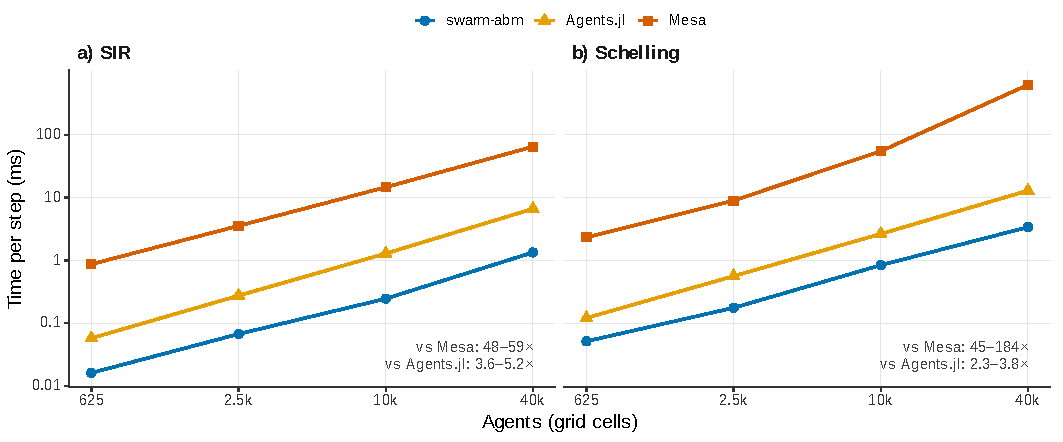
\includegraphics[width=\linewidth]{../figs/fig_performance.pdf}
\caption{Cross-engine per-step cost on spatial SIR (a) and Schelling (b),
median of three seeds, on log--log axes. swarm-abm is 2--5$\times$ faster than
Agents.jl and 45--184$\times$ faster than Mesa across both access patterns;
Agents.jl is itself 10--48$\times$ faster than Mesa, within its expected range,
confirming that the comparators are idiomatic. Raw values are in the repository.}
\label{fig:perf}
\end{figure}

In absolute terms, the engine sustains tens of millions of agent-steps per
second on a single thread (criterion microbenchmarks), so the cross-engine
margins reflect a genuinely fast core rather than a favourable model size.

\subsection{Scalability of the parallel decision phase}
The deterministic parallel decision phase (Section~\ref{sec:sync}) is the
engine's intra-step parallelism. Its benefit depends on whether per-agent
decisions are compute- or memory-bound, which we separate with a Game-of-Life
bench (250\,000 agents, 30 steps, median of 3 replicates) carrying a tunable
per-agent decision cost (Figure~\ref{fig:scaling}). When decisions are
compute-bound (the regime of agents with expensive logic such as utility
maximisation, perception or local optimisation, common in economic and social
ABM), the phase scales to $5.3\times$ on 16 threads. When they are
memory-bound (plain Life, a stencil), the speedup is a modest $1.6\times$:
bandwidth, not cores, is the limit, as expected for stencil computations.
Amdahl's law sets the ceiling (the apply phase is sequential), which is a
natural target for future work.

\begin{figure}[t]
\centering
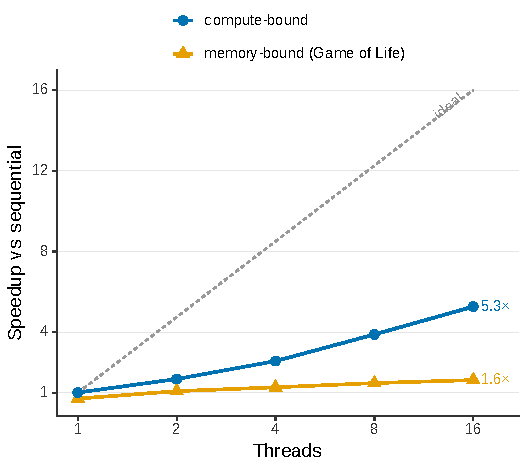
\includegraphics[width=0.62\linewidth]{../figs/fig_scaling.pdf}
\caption{Strong scaling of the parallel decision phase: speedup versus the
sequential run as threads increase, for compute-bound and memory-bound
per-agent decisions, with the ideal linear reference. Compute-bound decisions
scale to $5.3\times$ on 16 threads; memory-bound (plain Game of Life, a stencil)
saturate at $1.6\times$ as memory bandwidth, not cores, becomes the limit.}
\label{fig:scaling}
\end{figure}

Combined with the single-thread advantage over Agents.jl, the parallel decision
phase widens the gap precisely where intra-step parallelism pays, namely
expensive per-agent decisions.

\section{Application: spatial debris-flow simulation}
\label{sec:app}

To exercise the engine on a real, validated problem rather than a textbook one,
we re-implemented a published spatial model of debris flows (the 2015 Atacama
event, Chile) on swarm-abm, faithfully porting a Mesa/Python original
\cite{debrisflow2026}. The port reproduces the original distributionally on
identical inputs while running about $100\times$ faster (from $130$--$240$~s to
$1.2$--$4$~s per run on a $31.8$-million-cell domain). It also recovers
reproducibility the original lacked: the original drew from an unseeded
global generator, so its runs could not be replicated.

The point of the application is not the geomorphology but what the engine's
throughput \emph{enables} methodologically. Two studies that were impractical in
the original become routine:
\begin{itemize}
  \item \textbf{Robust calibration.} Differential Evolution
  \cite{storn1997differential} over the ported model, parallelised across cores,
  fits the model in $1$--$5$~min where the Python equivalent would take
  $11$--$34$~h ($\sim$$400\times$). Crucially, the cheap runs let us calibrate
  against a multi-seed objective and so detect and correct an over-fit to a
  single seed that single-run calibration hides.
  \item \textbf{A selection-and-comparison procedure for calibrators.} Because a
  full calibration is now minutes, we compare five metaheuristics
  (Differential Evolution, a genetic algorithm, particle-swarm, simulated
  annealing, and Grey Wolf Optimisation \cite{mirjalili2014grey}) with
  statistical power ($5\times10$ runs, $7\,500$ simulations in $\sim$12~min,
  versus $\sim$80~h in Python), using a Friedman test
  ($\chi^2 = 14.3$, $p = 0.006$) and Wilcoxon--Holm post-hoc comparisons
  \cite{demsar2006statistical}. Grey Wolf Optimisation wins and leads
  out-of-sample. This is exactly the kind of rigorous comparison the cost of an
  interpreted engine ordinarily precludes.
\end{itemize}
The application thus illustrates the paper's thesis concretely: lowering the
cost per run by two orders of magnitude does not merely speed up an existing
study: it changes which studies, and which conclusions, are reachable.

\section{Accessibility and reproducibility}
\label{sec:access}

A fast engine is only useful if practitioners can drive it. swarm-abm exposes
its models to Python through native bindings: the simulation loop runs entirely
in compiled code while Python configures runs, retrieves time series for
analysis in the scientific-Python stack, and launches parameter sweeps that
execute in parallel with the interpreter lock released. Results match the native
engine bit-for-bit. For communication and teaching, the engine also compiles to
WebAssembly: canonical models run in the browser on a canvas, deterministically,
in a binary of about 68~kB. The engine is open source under a permissive licence
with continuous integration (build, lint, format, documentation, and the
no-default-features path for WebAssembly), and the exact version used here will
be archived with a citable DOI. % TODO: Zenodo DOI on release

\section{Discussion}
\label{sec:discussion}

\paragraph{Compute is not neutral.}
The application makes concrete a claim that is easy to state and easy to ignore:
the cost of a simulation is not a neutral implementation detail but a constraint
on the science. We showed two cases where lowering it changed the conclusion,
not just the runtime: a robust calibration that overturns a single-seed
over-fit, and a statistically powered optimiser comparison that an interpreted
engine could not afford. Performance, here, is a methodological enabler, which
is why we frame it as a pillar rather than the headline.

\paragraph{Determinism as a methodological requirement.}
We have treated bit-level reproducibility not as an engineering nicety but as a
requirement of a credible computational science, and shown that it can be
guaranteed rather than hoped for: deterministic across seeds, across machines
(x86-64 and WebAssembly), and across thread counts. The type-enforced
synchronous update is the kernel that makes the parallel case hold, turning a
correctness proof into a reproducibility guarantee.

\paragraph{Relation to other engines.}
swarm-abm occupies the same niche as Agents.jl, a fast, single-machine,
general ABM framework, and is faster on our benchmarks while adding
deterministic parallelism and a WebAssembly target. It is complementary to
distributed and GPU engines: Repast HPC \cite{collier2013repast} targets
clusters and FLAME GPU \cite{richmond2023flamegpu} targets the GPU, regimes we
do not address. Standard model-description practice such as the ODD protocol
\cite{grimm2006odd} is orthogonal and compatible.

\paragraph{Limitations.}
Defining a new model requires writing Rust, a higher barrier than NetLogo's or
Mesa's; the Python bindings mitigate this for users who run existing models but
not for those who author new ones. The deterministic-parallelism guarantee
applies to the synchronous decision phase; the apply phase is still sequential,
which both bounds parallel speedup (Amdahl) and is the obvious next target,
since in many models the apply phase writes to disjoint locations and could be
parallelised under a similar disjointness guarantee.

\section{Conclusions}
\label{sec:conclusion}

We presented swarm-abm, a spatial agent-based simulation engine organised around
determinism by construction. Its kernel is a type-enforced immutability that
simultaneously proves the synchronous update correct and makes it safe to
parallelise, yielding parallel execution that is bit-for-bit identical to
sequential and reproducible across machines, properties we validated with
PractRand and across x86-64 and WebAssembly. The engine is fast where it matters,
2--5$\times$ over Agents.jl and 45--184$\times$ over Mesa on canonical models,
with intra-step parallelism that scales $\sim$5$\times$ on 16 cores for
compute-bound decisions, and we demonstrated on a real debris-flow application
that this performance enlarges the set of tractable analyses rather than merely
accelerating existing ones. The contribution is not speed alone but
\emph{reproducible} speed: a simulation engine on which results can be trusted to
replicate, exactly, as they are scaled.

\section*{Declaration of generative AI use}
% TODO (Elsevier, obligatorio si aplica).

\section*{Data availability}
The engine, the benchmark mirrors, and the validation scripts are openly
available (Section~\ref{sec:access}); a versioned archive with a citable DOI
will accompany publication.

\bibliography{refs}

\end{document}
